\documentclass[12pt]{report}
\usepackage[english]{babel}
\usepackage[utf8]{inputenc}

\usepackage[dvipsnames]{xcolor}

\usepackage{array}
\newcolumntype{L}{>{\centering\arraybackslash}m{3cm}}

\usepackage{algorithm}
\usepackage{algpseudocode}
\usepackage{caption}

\usepackage{graphicx}
\usepackage{csquotes}

\title{Advanced Machine Learning\\Final Report}

\author{Shayan Amani}

\date{\today}

\begin{document}
\maketitle

\chapter{Problem Definition}
Presenting an optimum policy to control a specific invasive species, Frangula alnus so called, glossy buckthorn. For the sake of simplicity, a grid environment of 3x3 has been considered. 

Simulator-generated samples of history of measures and consequences are provided in a dataset. Dataset is consisted of the following columns:
\begin{itemize}
    \item \textbf{V1}: year number of the sample. from 1 to 200 which means simulator run through a span of 200 years.
    \item: \textbf{pop\_1} to \textbf{pop\_9}: population of the plant in each cells.
    \item: \textbf{sbank\_1} to \textbf{sbank\_9}: number of plant's seeds in each cells.
    \item: \textbf{actions}: taken action for each year of samples.
    \item: \textbf{rewards}: observed reward after applying the action.
\end{itemize}

\chapter{Previous Works}
We have two different point of view to look at this problem. Firstly a batch reinforcement learning problem and secondly




\chapter{Proposed and Implemented Method}
Considering this sample-based problem I have picked and implemented a deep reinforcement learning approach, namely Deep Q-Networks (DQN). The elements of this method are explained in the following sections.

This needs to be mentioned that I have examined different method which are excelled in the literature. One of these methods is Deep Deterministic Policy Gradient (DDPG). According 

\section{Algorithm}
The whole algorithm is described in Algorithm \ref{alg:DQN}.

\begin{algorithm}[H]
\caption{DQN algorithm in batch mode}
\label{alg:DQN}
\begin{algorithmic}[1]
    \State Init D \Comment{\textcolor{BlueViolet}{replay memory}}
    \State Init Q \Comment{\textcolor{BlueViolet}{Q-table w/ random weights}}
    \State \textcolor{OrangeRed}{Get} or Observe $s_0$ \Comment{\textcolor{BlueViolet}{the initial state}}
    \For{each episode}
        \For{samples in each episode}
            \State \textit{\textcolor{OrangeRed}{- skip $\epsilon$-greedy exploration}}
            \State $a = argmax_a Q(s,a)$
            \State \textit{\textcolor{OrangeRed}{- skip applying action $a$ to the environment}}
            \rlap{\smash{$\left.\begin{array}{@{}c@{}}\\{}\\{}\end{array}\color{BlueViolet}\right\}%
              \color{BlueViolet} experience$}}
            \State \textcolor{OrangeRed}{Get} or Observe $r, s'$
            \State Store the \textbf{experience} $<s, a, r, s'>$ in replay memory $D$
            \State \textit{Random} \textbf{sampling} from $D$ $<ss, aa, rr, ss'>$  \Comment{\textcolor{BlueViolet}{[mini]-batch}}
            \If{$ss' \neq $ terminal state} \Comment{\textcolor{BlueViolet}{target for each mini-batch}}
                \State $tt = rr + \gamma max_{aa'} Q(ss', aa')$
            \Else
                \State $tt = rr$
            \EndIf
            \State Train the network
        \EndFor    
    \EndFor
\end{algorithmic}
\end{algorithm}

\section{Experience Replay}
DQN is mostly relied on a stabilization technique with neural networks, called Experience replay. Experience replay is a memory abstraction which $n$ past samples are stored in this memory and then we use it later to draw samples from it on a randomized basis. 



% 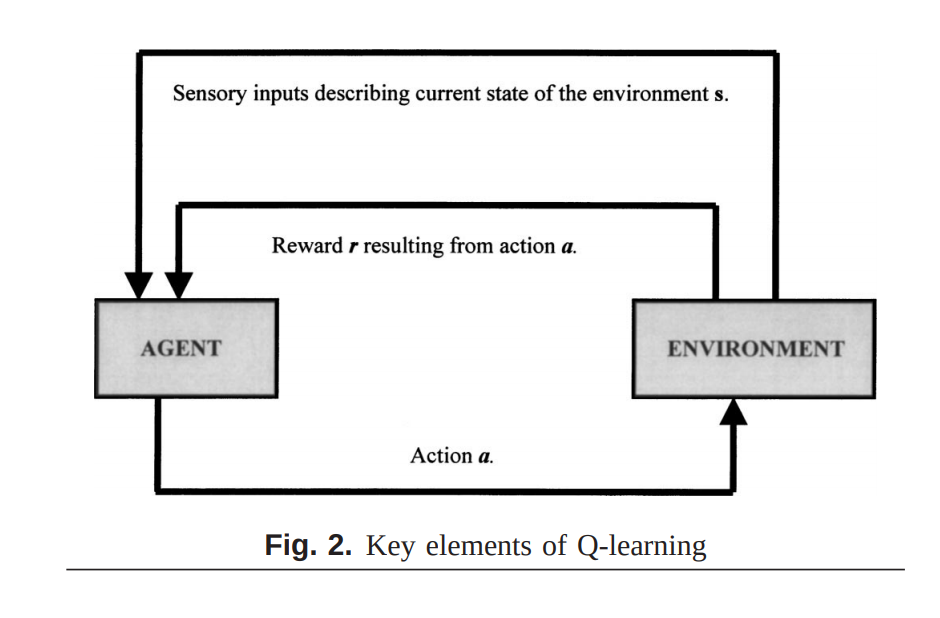
\includegraphics[width=1\columnwidth]{elements.png}


\end{document}